\begin{block}{Ausgangspunkt}
Die Metaanalysen belegen die positiven Effekte kooperativer Lehr- und Lernmethoden hinsichtlich der Lernleistungen (Johnson, Johnson \& Stanne, 2000; Rohrbeck, Ginsburg-Block, Fantuzzo \& Miller, 2003; Slavin 1995). Die berichteten Effekte variieren stark. Untersuchungen mit jüngeren Schülerinnen und Schülern werden relativ selten durchgeführt. 

Ziel der Studie ist den Prozess des Wissenserwerbs beim kooperativen Lernen bei jüngeren Schülerinnen und Schülern näher zu untersuchen. Dazu wird die kooperative Methode des Gruppenpuzzles (Aronson, Blaney, Stephan, Sikes, \& Snapp, 1978) in der dritten Klassenstufe eingesetzt.
\end{block}


\begin{block}{Gruppenpuzzle}

\begin{figure}
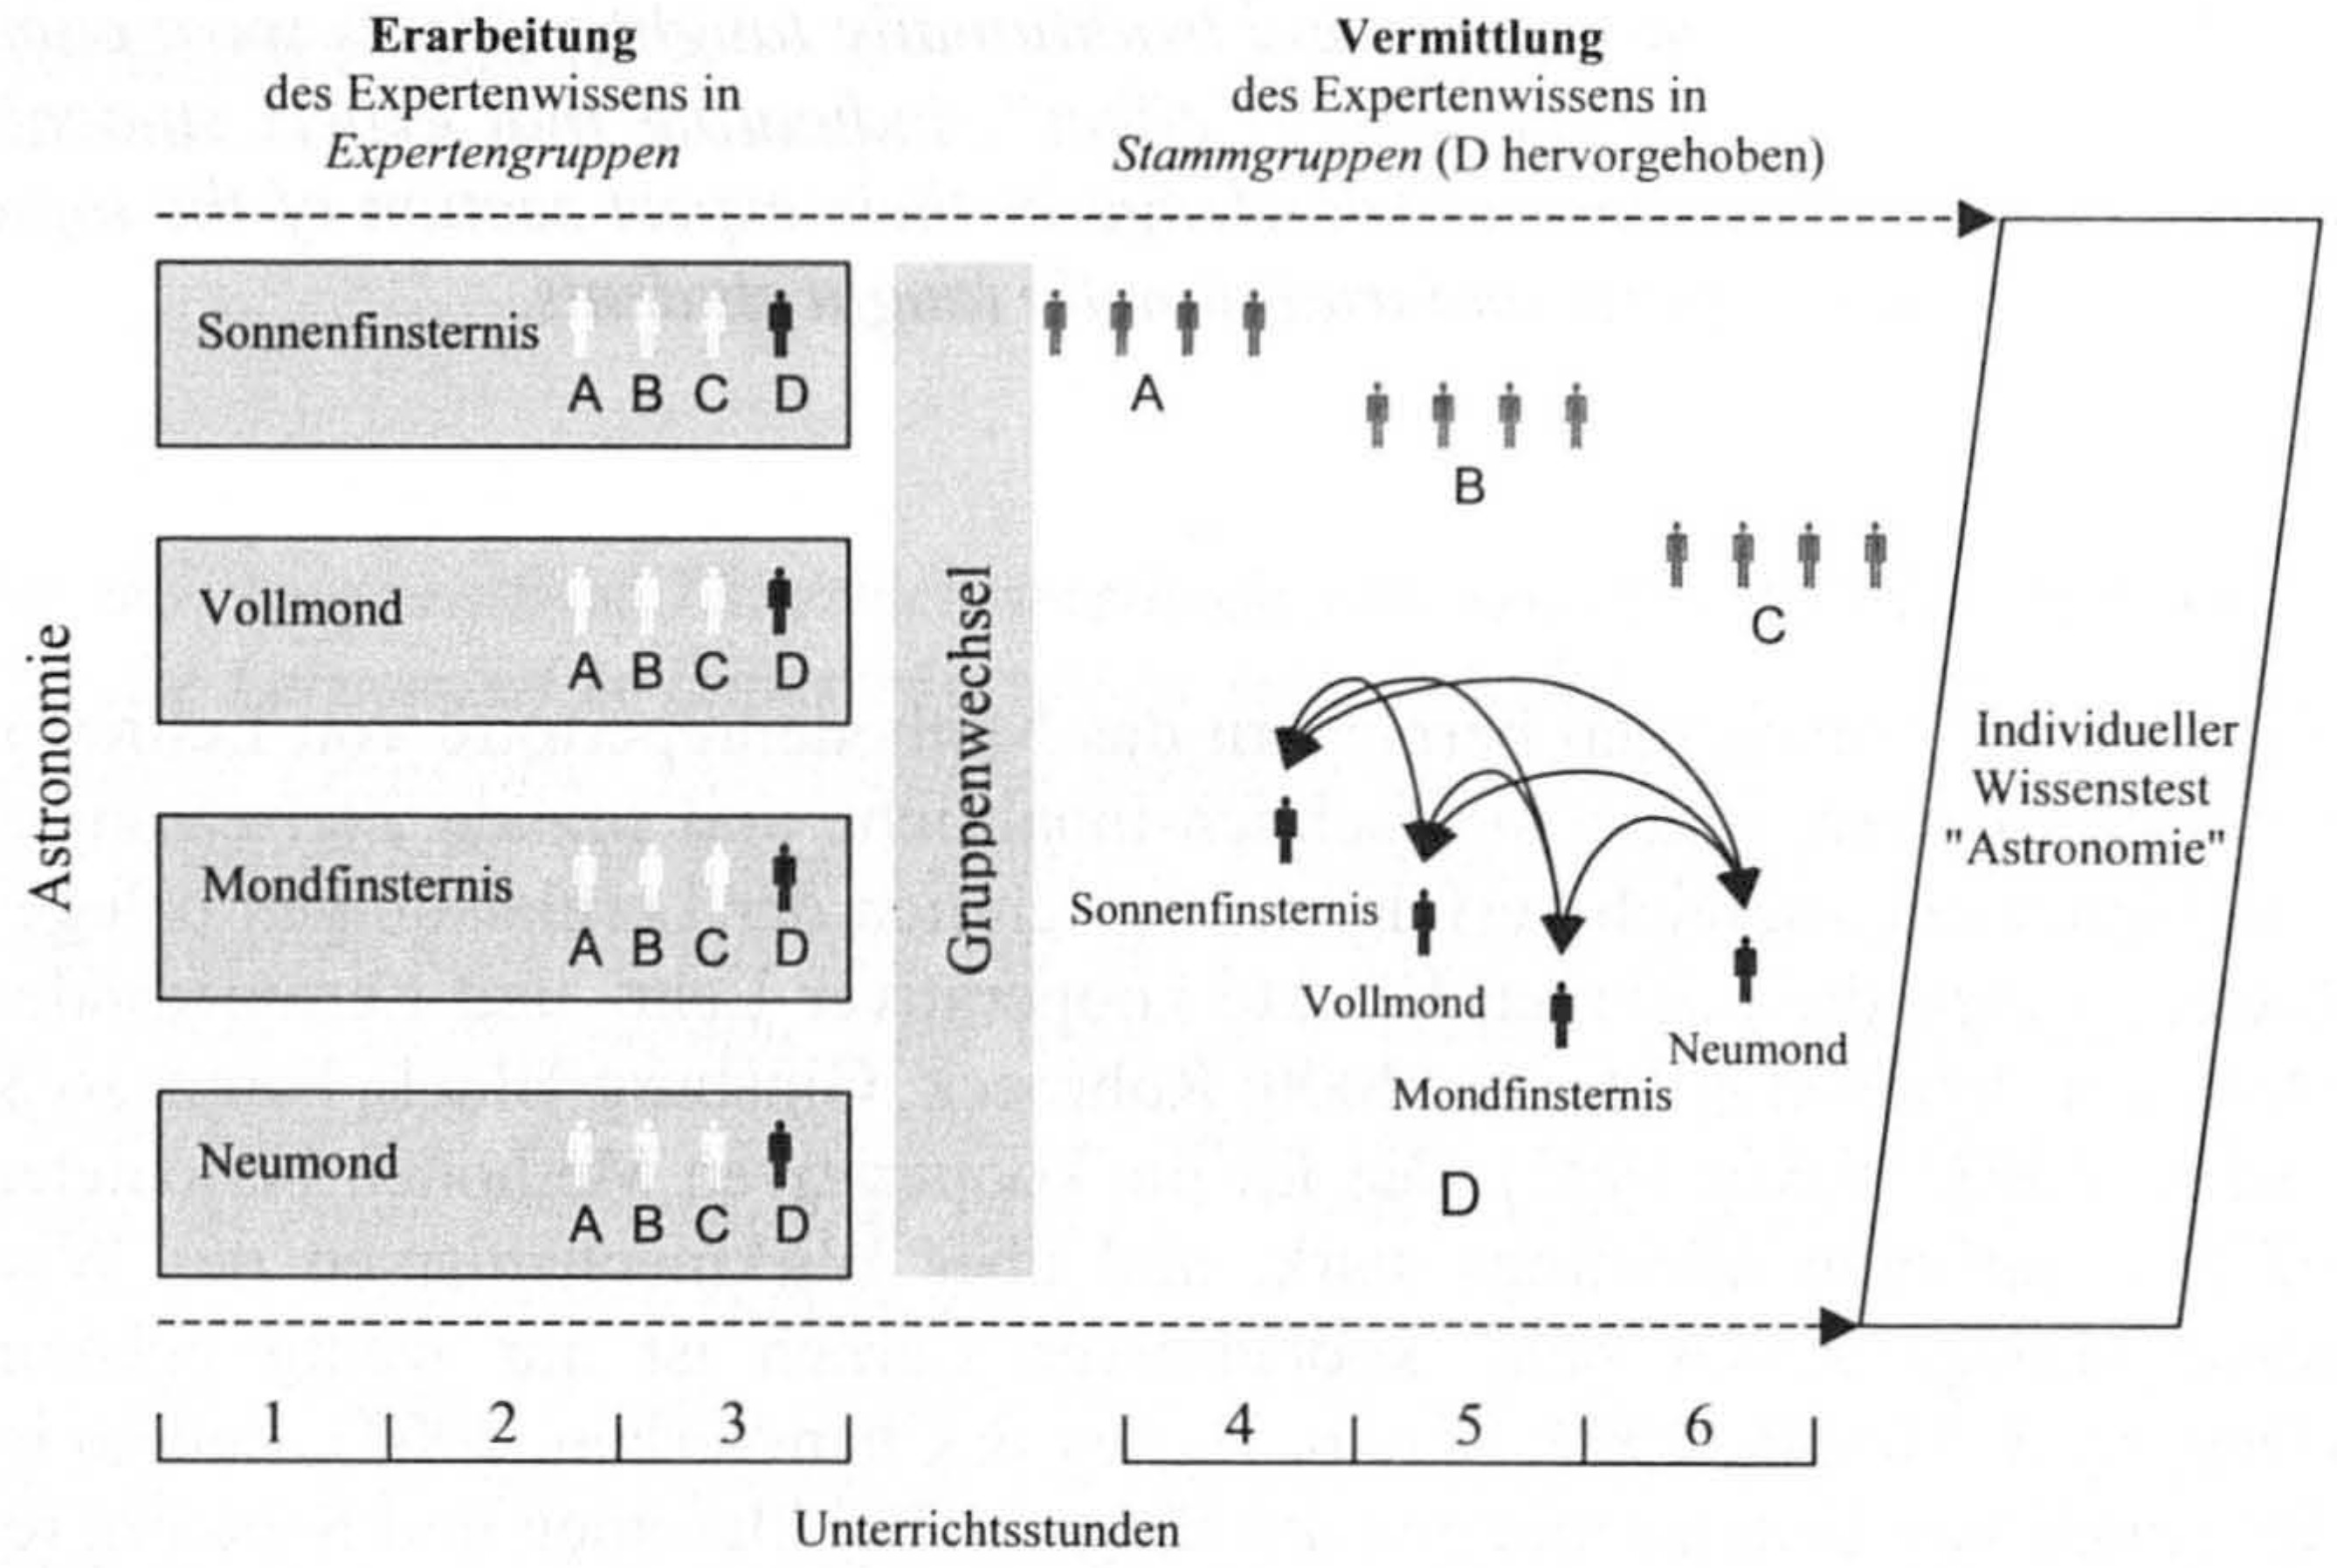
\includegraphics[width=0.67\linewidth]{experteneffekt.jpg}
\caption{Wissenserwerbsprozess im Gruppenpuzzle in einer sechsstündigen Sachunterrichtseinheit der Primarstufe}
\end{figure}

\textbf{Erarbeitunsphase} Lernstoff wird in verschiedene Teilgebiete aufgeteilt. Jede Schülerin bzw. jeder Schüler einer Klasse, erarbeitet jeweils ein Teilgebiet. 

\textbf{Vermittlungsphase} die Teilgebiets-Experten wechseln in ihre jeweilige Stammgruppen zurück und geben das neu erworbene Wissen an die Nichtexperten ihrer Gruppe weiter. 

\textbf{Experteneffekt} Diskrepanz zwischen den Lernfortschritten von Experten und Nichtexperten.  
\end{block}


\begin{alertblock}{Fragestellungen}
\begin{enumerate}
\item Sind die Lernleistungen der Gruppenpuzzleexperten in ihrem eigenen Expertenbereich höher als die von Nichtexperten und Kindern im herkömmlichen Unterricht in diesem Bereich?
\item Sind die Lernleistungen der Nichtexperten im Gruppenpuzzle höher als im herkömmlichen Unterricht?
\item Lässt sich das kooperative Arbeiten durch den wiederholten Einsatz der Methode verbessern?
\end{enumerate}
\end{alertblock}
